%------------------------------------------------
\chapter{Resultados Observados}\label{Resultados}
%---------------------------------------------------------

\section{Introdução}
Este capítulo apresenta os resultados observados e as análises realizadas a partir dos testes nos módulos implementados. A divisão das seções é a mesma anteriormente apresentada para a apresentação dos resultados individualmente. Finalmente, é realizada uma análise geral do sistema como um todo.

Nas simulações realizadas, algumas adaptações foram feitas no esquemático da Figura \ref{fig:schematic}. A \textit{Região 1} foi modelada como uma fonte de sinal senoidal, simulando a portadora na frequência de $915~MHz$, sem informação modulada. A temperatura de simulação, quando não informado diferente, é de $27~^{\circ}$. A \textit{Região 2} é externa ao \textit{chip}, uma vez que a tecnologia utilizada não previa diodos dos tipos \textit{Schottky} e Zener. Para simulá-los, foram utilizados modelos implementados em \textit{VerilogA}, uma linguagem de descrição de hardware analógico. Finalmente, o valor de capacitância utilizado na maioria dos testes foi de 1 pF, a fim de permitir que as simulações fossem realizadas em tempo hábil. Caso o contrário não seja dito, esse valor deve ser assumido.


\section{Retificador}
% TODO - Testes: Periodic Steady-State (PSS) e Periodic S-Parameter (PSP)
O retificador foi implementado tal como é mostrado nas Figuras \ref{fig:rectifier_cell} e \ref{fig:rectifier_6_cells}. Foi utilizada uma fonte senoidal de $1~V_{pp}$ e frequência de $915~MHz$ para a simulação do sinal de entrada. Esse sinal é distribuído ao longo das células e é amplificado em cada ciclo de retificação.

Na Figura \ref{fig:rectifier_cell_transient} é apresentado o resultado de simulação transiente realizado para uma célula do retificador, com uma carga de 1 pF. Nos primeiros ciclos de carga, o capacitor de 250 fF, inicialmente descarregado, recebe energia da onda incidente, carregando-se a cada ciclo, até a saturação. Neste caso, esse valor é o mesmo das quedas de tensão sobre os dois diodos MOS da célula.

\begin{figure}[!htb]
	\caption{\label{fig:rectifier_cell_transient}Simulação transiente da célula do retificador}
	\begin{center}
		\includegraphics[width=.95\linewidth]{rectifier_cell_transient.png}
	\end{center}
	\legend{Fonte: autor}
\end{figure}

Na simulação, observa-se que o sinal retificado converge a um valor médio superior ao nível AC da fonte de entrada. Ainda há, contudo, uma oscilação no sinal retificado. Nos instantes finais de simulação seus valores máximo e mínimo são, respectivamente, $0,6771~V$ e $0,6590~V$.

O nível de amplificação da célula é dependente das dimensões dos transistores e capacitores empregados. Segundo \citeonline{ALLEN:2002}, a resistência desses dispositivos é inversamente proporcional à relação $\dfrac{W}{L}$ do transistor, para baixos níveis de tensão $v_{DS}$. Um aumento nessa característica diminui a resistência da carga ativa e, portanto, a queda de tensão sobre os elementos.

Outra característica dependente das dimensões do transistor é a variação da amplitude do sinal de saída. À medida que a resistência dos elementos diminui, a impedância do sistema também é reduzida, permitindo maior excursão do sinal de saída.

O retificador foi desenvolvido com a implementação, em série, de 6 células de retificação, conforme apresentado na Figura \ref{fig:rectifier_6_cells}. Na Figura \ref{fig:rectifier_transient} é mostrado o resultado da resposta transiente do retificador sem carga. É possível observar a convergência do sinal retificado a um nível médio de, aproximadamente, $3,74~V$. O sinal retificado ainda apresenta oscilação, variando de $3,733~V$ a $3,748~V$ instantes finais. Na Figura \ref{fig:rectifier_transient_2} é possível observar a resposta do retificador com o ajuste externo, como mostrado no esquemático da Figura \ref{fig:schematic}. O sinal retificado, nesse caso, possui maior excursão que o caso sem carga, devido à inserção dos elementos externos ao retificador, que diminuem a impedância de saída do módulo. Nos instantes finais o sinal retificado oscila de $3,677~V$ a $3,747~V$, implicando numa tensão média de, aproximadamente, $3,71~V$, ligeiramente inferior ao caso sem carga. Finalmente, a tensão não regulada do sistema é observada constante e, na simulação realizada, tem o valor de $3,575~V$. Um diodo zener é utilizado para evitar que níveis de tensão superiores a $3,6~V$ sejam alcançados.

\begin{figure}[!htb]
	\caption{\label{fig:rectifier_transient}Simulação transiente do retificador sem ajuste externo}
	\begin{center}
		\includegraphics[width=.95\linewidth]{rectifier_transient.png}
	\end{center}
	\legend{Fonte: autor}
\end{figure}

\begin{figure}[!htb]
	\caption{\label{fig:rectifier_transient_2}Simulação transiente do retificador com ajuste externo}
	\begin{center}
		\includegraphics[width=.95\linewidth]{rectifier_transient_2.png}
	\end{center}
	\legend{Fonte: autor}
\end{figure}

Um teste transiente realizado no retificador mostrou que para que o capacitor de carga atinja o nível de tensão nominal de $3,5~V$, são necessários $239,1~\mu W$ na entrada. Para a saída, são fornecidos $18,52~\mu W$. Isso implica num rendimento de, aproximadamente, $7,75\%$ para o sistema. Esse valor está aquém do observado na literatura, indicando que melhorias podem ser feitas nesse módulo.


%\section{Modulador}
%O modulador foi implementado como descrito no Capítulo anterior. Este módulo foi projetado de forma bastante simples e não há muito o que se discutir a respeito. Seu funcionamento, como descrito, consiste em modular o sinal da portadora de acordo com o controle proveniente do núcleo digital do sistema.

%O núcleo digital provê a informação a ser modulada, que serve como controle do transistor modulador. A modulação utilizada é do tipo {ASK}. A codificação dos \textit{bits} de nível lógico alto ou baixo é realizada com a variação de amplitude da portadora. O \textit{bit} $0$ é modulado com maior tempo de alta que o \textit{bit} $1$. A duração do pulso positivo determina se cada \textit{bit} é zero ou um. A relação entre eles é de, no mínimo, 1,5:1 e, no máximo, 2:1 \cite{YEAGER:2009}.


\section{Referencial de Tensão}
Os referenciais de tensão foram implementados como mostrado na Figura \ref{fig:bandgap}. Para minimização das correntes no circuito, foi utilizada largura mínima em todos os transistores. A variação de seus comprimentos permitiu a obtenção de distintos níveis de referência. Nas Figuras \ref{fig:bandgap_dc_0_7} e \ref{fig:bandgap_dc_1_2} são apresentados os resultados de simulações {CC} para os circuitos referenciais de tensão de $0,7~V$ e $1,2~V$, respectivamente.

\begin{figure}[!htb]
	\caption{\label{fig:bandgap_dc_0_7}Simulação {CC} do circuito referencial de tensão de $0,7~V$}
	\begin{center}
		\includegraphics[width=.95\linewidth]{bandgap_dc_0_7.png}
	\end{center}
	\legend{Fonte: autor}
\end{figure}

\begin{figure}[!htb]
	\caption{\label{fig:bandgap_dc_1_2}Simulação {CC} do circuito referencial de tensão de $1,2~V$}
	\begin{center}
		\includegraphics[width=.95\linewidth]{bandgap_dc_1_2.png}
	\end{center}
	\legend{Fonte: autor}
\end{figure}

Nos gráficos das simulações {CC} realizadas, é possível observar que as respostas dos módulos mudam de comportamento a partir de um certo nível. Para o referencial de $0,7~V$ este ponto está em torno de $0,8~V$. A partir daí a resposta assume um comportamento ainda crescente, porém com inclinação bastante reduzida, quase nula. Já para o referencial de $1,2~V$ o ponto é, aproximadamente, $1,3~V$. A inclinação da curva após este ponto é pequena, mas visivelmente existente. Contudo, numa simulação para $V_{nr}$ até $3,8~V$, a referência de tensão chega a um máximo de $1,241~V$, apenas 3,42\% superior ao valor desejado.

\begin{figure}[!htb]
	\caption{\label{fig:bandgap_temp_0_7}Simulação de variação temperatura do circuito referencial de tensão de $0,7~V$}
	\begin{center}
		\includegraphics[width=.95\linewidth]{bandgap_temp_0_7.png}
	\end{center}
	\legend{Fonte: autor}
\end{figure}

\begin{figure}[!htb]
	\caption{\label{fig:bandgap_temp_1_2}Simulação de variação temperatura do circuito referencial de tensão de $1,2~V$}
	\begin{center}
		\includegraphics[width=.95\linewidth]{bandgap_temp_1_2.png}
	\end{center}
	\legend{Fonte: autor}
\end{figure}

Nas Figuras \ref{fig:bandgap_temp_0_7} e \ref{fig:bandgap_temp_1_2} são apresentadas as respostas dos sistemas para simulações de variação de temperatura, sob a tensão não-regulada de $3,5~V$. Como esperado, os sistemas apresentam pouca variação com a temperatura, principalmente o referencial de $1,2~V$. Esse resultado é observado devido à soma de componentes {PTAT} e {CTAT}, como explicado por \citeonline{MARTIN:1997}. Contudo, em nenhuma das duas implementações se conseguiu independência completa da temperatura. Para o referencial de tensão de $0,7~V$, houve uma variação percentual de, aproximadamente, $14,29~\%$ em torno do valor desejado. Já para o referencial de $1,2~V$, essa variação foi de $4,17~\%$.

Observou-se a potência necessária por cada um dos circuitos referenciais para seu funcionamento. As correntes observadas para o ponto de operação com $V_{nr}~=~3,5~V$ foram de, aproximadamente, $318~nA$ e $49~nA$ para os referenciais de $1,2~V$ e $0,7~V$, respectivamente. Nesse caso, as potências dissipadas, tomadas como $V_{nr}~\cdot~I_{alimentação}$ são iguais a $1,113~\mu W$ e $0,172~\mu W$, respectivamente.

Uma possível implementação para o referencial de $0,7~V$ a partir do inicial de $1,2~V$ seria a utilização de um divisor de tensão com resistências precisas. Um possível circuito para este fim é apresentado na Figura \ref{fig:0_7_ref_divider}. Os valores de resistência foram escolhidos de forma a minimizar a dissipação de potência por efeito Joule. Da forma apresentada, as perdas nos resistores seriam da ordem de $0,168~\mu W$. Essa dissipação é, virtualmente, igual à potência consumida pelo módulo referencial implementado. Devido à maior simplicidade desse sistema, a propensão a erros é menor, bastando que haja cuidado na inserção dos resistores no \textit{layout} do projeto e que sejam utilizados dispositivos de precisão. A área ocupada por ambos os modelos propostos é similar, tendo sua maior parte devida às altas resistências utilizadas.

\begin{figure}[!htb]
	\caption{\label{fig:0_7_ref_divider}Possível topologia para geração do referencial de $0,7~V$}
	\begin{center}
		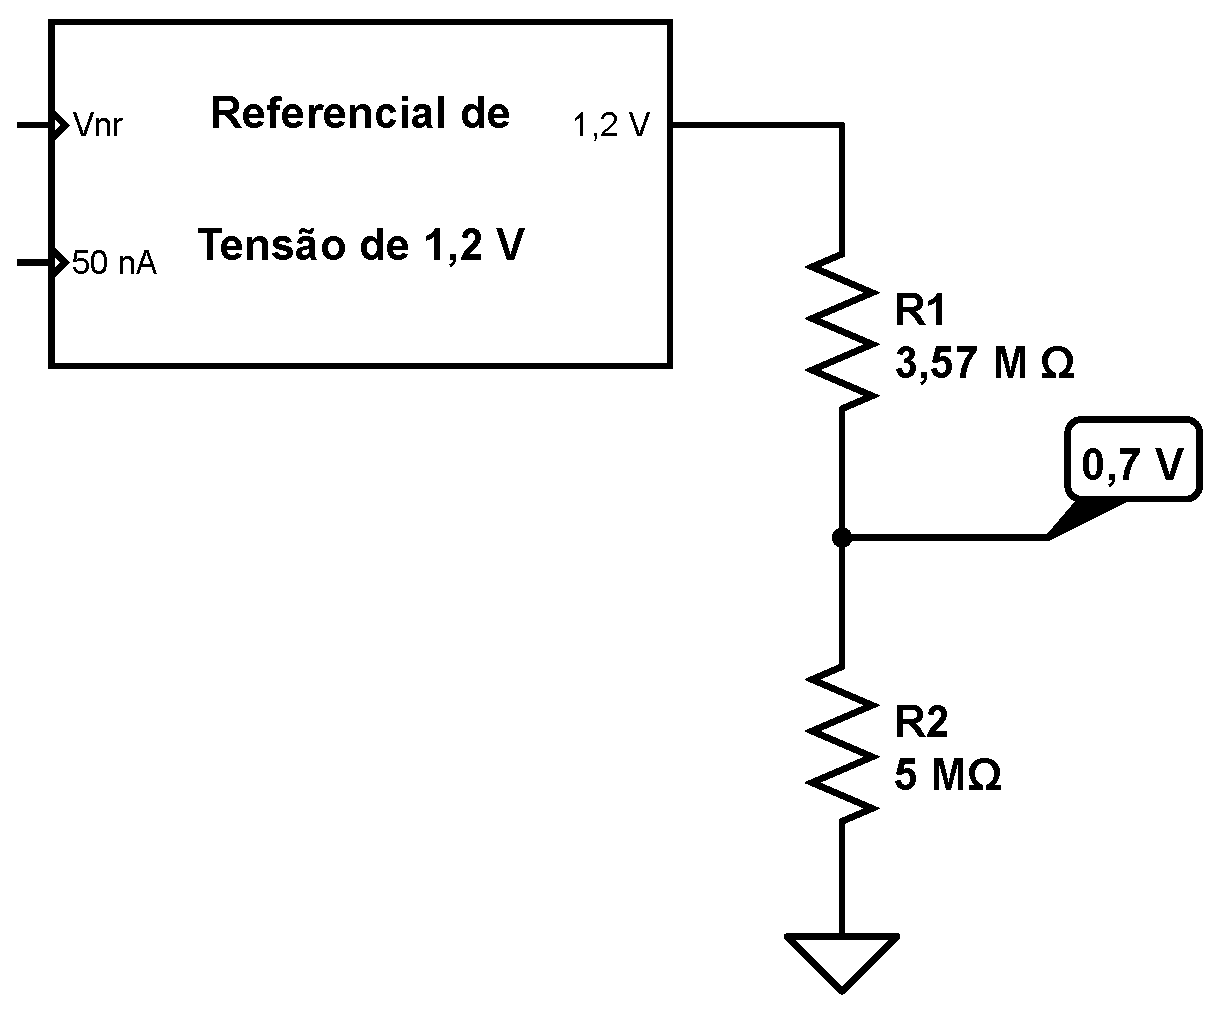
\includegraphics[width=.7\linewidth]{alternative-0_7-v-reference.eps}
	\end{center}
	\legend{Fonte: autor}
\end{figure}

A escolha da topologia utilizada para a implementação do referencial de tensão de $0,7~V$ levou em consideração, também, o fato de que é necessária uma tensão de polarização para a configuração em cascata do regulador de tensão. Esse nível é o mesmo utilizado para polarizar os transistores do referencial de tensão.


\section{Referencial de Corrente}
O referencial de corrente foi implementado como mostrado na Figura \ref{fig:bias_current}. O circuito começa a fornecer a corrente de referencial quando a tensão não-regulada alcança o nível de, aproximadamente, $550~mV$. A alta impedância do sistema em cascata é responsável pela manutenção da constância do valor de corrente de saída. Esse comportamento é ilustrado na Figura \ref{fig:bias_current_dc}, que expõe o resultado da simulação {CC} do circuito gerador de referencial de corrente, com variação da tensão não-regulada de $0~V$ a $3,8~V$. O valor de corrente observado para $V_{nr}~=~550~mV$ é de $49~nA$. Para $V_{nr}~=~3,8~V$, a esse valor é de $50,34~nA$.

\begin{figure}[!htb]
	\caption{\label{fig:bias_current_dc}Resultado da simulação {CC} do referencial de corrente}
	\begin{center}
		\includegraphics[width=.95\linewidth]{bias_current_dc.png}
	\end{center}
	\legend{Fonte: autor}
\end{figure}

\begin{figure}[!htb]
	\caption{\label{fig:bias_current_temp}Resultado do teste de variação de temperatura do referencial de corrente}
	\begin{center}
		\includegraphics[width=.95\linewidth]{bias_current_temp.png}
	\end{center}
	\legend{Fonte: autor}
\end{figure}

Na Figura \ref{fig:bias_current_temp} é apresentado o resultado da simulação {CC} sob tensão constante, fazendo variar a temperatura de operação do sistema. O gráfico apresentado indica que não há independência de temperatura no sistema proposto. A variação foi de, aproximadamente, $314~\%$ em torno do valor desejado. Essa é uma característica não ideal e que deve ser melhorada em futuras abordagens do problema. A curva de relação com a temperatura indica que o sistema é do tipo {PTAT}. Uma possível forma de se obter independência da temperatura, como explicado por \citeonline{MARTIN:1997}, é buscar um nível de tensão {CTAT} e utilizá-lo para neutralizar o incremento da saída com a temperatura.

O circuito implementado, na tensão de alimentação de $3,5~V$ consome $2,514~\mu A$, segundo a simulação {CC} realizada. Isso implica numa potência necessária de $8,799~\mu W$ para o funcionamento do módulo, com as cinco fontes de corrente operando em valor nominal.


\section{Regulador de Tensão}
Os reguladores de tensão utilizados neste trabalho foram implementados como exposto na Figura \ref{fig:regulator}. Foram utilizados dois módulos, um para a regulação da tensão de $0,7~V$ e outro para $1,2~V$. A única diferença de projeto entre os módulos se dá no transistor de passagem, que serve como queda de potencial entre a tensão de não-regulada e a saída do sistema. Para esse transistor foi utilizado um alto valor de largura, de modo a facilitar a passagem de corrente e reduzir as perdas por efeito Joule. Sua relação $\dfrac{W}{L}$ foi definida para cargas de $6~\mu A$ e $10~\mu A$, respectivamente. Esses valores foram arbitrariamente escolhidos e devem ser adaptados à aplicação, de acordo com a carga que será utilizada. Ajustes finos na simulação permitiram a obtenção de valores mais precisos.

\begin{figure}[!hb]
	\caption{\label{fig:regulator_dc_0_7}Resultado da simulação {CC} do regulador de tensão de $0,7~V$}
	\begin{center}
		\includegraphics[width=.95\linewidth]{regulator_dc_0_7.png}
	\end{center}
	\legend{Fonte: autor}
\end{figure}

\begin{figure}[!hb]
	\caption{\label{fig:regulator_dc_1_2}Resultado da simulação {CC} do regulador de tensão de $1,2~V$}
	\begin{center}
		\includegraphics[width=.95\linewidth]{regulator_dc_1_2.png}
	\end{center}
	\legend{Fonte: autor}
\end{figure}

Nas Figuras \ref{fig:regulator_dc_0_7} e \ref{fig:regulator_dc_1_2} são apresentados os resultados de simulação {CC} realizados com os módulos implementados. Como referencia de tensão, utilizou-se o módulo gerador de tal referencial, tratado neste capítulo. Foi, também, utilizado o módulo referencial de corrente, a fim de fornecer o nível de polarização do estágio amplificador para os reguladores.

Nos gráficos, observa-se o comportamento quase constante dos valores de tensão regulada, para $V_{nr}~\geq~2,5~V$. É percebida uma tendência à queda abrupta da tensão regulada do regulador de $0,7~V$ para valores de tensão não-regulada superiores a $3,5~V$. Em uma situação prática, o nível de tensão pode ser fixado em um valor arbitrário definido pelo projetista, como $3~V$ ou $3,3~V$, onde os níveis regulados estão dentro do desejado.

\begin{figure}[!htb]
	\caption{\label{fig:regulator_temp_0_7}Resultado da simulação de temperatura do regulador de tensão de $0,7~V$}
	\begin{center}
		\includegraphics[width=.95\linewidth]{regulator_temp_0_7.png}
	\end{center}
	\legend{Fonte: autor}
\end{figure}

\begin{figure}[!htb]
	\caption{\label{fig:regulator_temp_1_2}Resultado da simulação de temperatura do regulador de tensão de $1,2~V$}
	\begin{center}
		\includegraphics[width=.95\linewidth]{regulator_temp_1_2.png}
	\end{center}
	\legend{Fonte: autor}
\end{figure}

Nas Figuras \ref{fig:regulator_temp_0_7} e \ref{fig:regulator_temp_1_2} são expostas as respostas dos sistemas para simulações de variação da temperatura, sob a tensão não-regulada de $3,5~V$. O circuito de simulação foi o mesmo utilizado para a anteriormente apresentada. A variação da tensão com a temperatura foi de, aproximadamente, $100~\%$ e $91,67~\%$ para as regulações de $0,7~V$ e $1,2~V$, respectivamente. Contudo, observa-se que o comportamento com a variação da temperatura não é linear para toda a faixa de valores observada. Para valores muito baixos de temperatura, o comportamento do circuito é quase constante. Para o regulador de $0,7~V$, a partir dos $17~^{\circ}C$ percebe-se um aumento linear com o incremento da temperatura. Esse comportamento permanece até os $30~^{\circ}$, onde a curva muda de inclinação, permanecendo, porém, linear. Para o regulador de $1,2~V$, o mesmo comportamento geral é observado, com as mudanças de inclinação nas temperaturas de $13~^{\circ}$ e $27~^{\circ}$.

Tal como observado no referencial de corrente, os módulos aqui implementados apresentam comportamento {PTAT}, tendo seu valor aumentado com o aumento da temperatura. O comportamento desejado seria independência dessa variável, de modo que a previsão da saída do módulo fosse possível independentemente da circunstância em que o sistema se encontrasse. Uma possível solução para contornar esse problema seria análoga ao circuito referencial de tensão implementado. Seriam utilizados o sinal de polarização do transistor {M7} e outro sinal com o mesmo tipo de variação em função da temperatura ({PTAT} ou {CTAT}) como entradas em um amplificador operacional. O efeito similar dos dois sinais com a variação de temperatura seria anulado pelo amplificador. Sua saída seria, então, utilizada para polarizar o transistor {M7}.

Para a tensão nominal de testes $V_{nr}~=~3,5~V$, observou-se que o módulo regulador de $0,7~V$ drenava uma corrente de $6,138~\mu A$ na entrada, resultando numa demanda de $21,483~\mu W$. O módulo regulador de $1,2~V$, por sua vez, drenava $10,68~\mu A$, alimentado sob o mesmo nível de tensão, resultando numa demanda de $37,38~\mu W$.


\section{Sistema Completo}
O sistema exposto na Figura \ref{fig:schematic} foi montado a partir dos módulos básicos implementados, cujos comportamentos foram apresentados ao longo deste capítulo. A \textit{Região 1} do esquemático foi modelada como uma fonte senoidal de $1~V_{pp}$. O resultado obtido condiz, satisfatoriamente, com o esperado segundo a teoria e os projetos realizados. Algumas análises foram feitas em cima do sistema proposto. Elas são apresentadas a seguir.

Inicialmente, foram realizados testes com os componentes do circuito descarregados. Contudo, verificou-se que, devido à alta capacitância utilizada na \textit{Região 2}, o tempo necessário para a carga inicial dos capacitores do circuito era muito alta, inviabilizando a simulação completa do sistema. Isso se deve à alta resistência do diodo \textit{schottky}, que serve como elemento resistivo ao circuito de carga do capacitor. A resistência observada em simulação para esse elemento foi de, aproximadamente, $1,333~M\Omega$. Para uma capacitância de $10~\mu F$, a constante de tempo do sistema de carga seria, aproximadamente, $13,33 s$. Possíveis soluções para a diminuição do tempo necessário para a carga desse capacitor seriam a diminuição do valor de capacitância ou a redução da resistência série do circuito de carga, com a utilização de diodos \textit{schottky} em paralelo, por exemplo. O tempo necessário para a carga das capacitâncias do sistema é reduzido após a primeira utilização. Os capacitores não são descarregados por completo, o que facilita o processo de cargas futuras.

\begin{figure}[!h]
	\caption{\label{fig:all_modules_trans_50us}Resultado da simulação transiente do sistema completo}
	\begin{center}
		\includegraphics[width=.95\linewidth]{all_modules_trans_50us.png}
	\end{center}
	\legend{Fonte: autor}
\end{figure}

Uma vez obtida a tensão não-regulada que serve como fonte de alimentação para os demais módulos do sistema, o comportamento de cada módulo individualmente é o mesmo realizado nas seções anteriores deste capítulo. Na Figura \ref{fig:all_modules_trans_50us} é apresentado o resultado da simulação transiente do sistema para $50~\mu s$. No gráfico apresentado é possível observar a constância dos valores de interesse. Para essa simulação, foram definidos os níveis de tensão iniciais para os nós do retificador e da fonte não-regulada. Para esta foi utilizado o valor de $3,5~V$. Os valores de tensão dos nós do retificador foram coletados da análise transiente desse módulo isoladamente. O valor de capacitância utilizado para a fonte não-regulada foi de $10~\mu F$. A Tabela \ref{tab:all_modules_trans_50us} apresenta os valores do gráfico numa forma mais direta.

\begin{table}[!htb]
	\centering
	\caption{\label{tab:all_modules_trans_50us}Valores observados na simulação do sistema completo}
	\begin{tabular}{c|cc}
		\textbf{Grandeza} & \textbf{Valor} & \textbf{Unidade} \\
		\hline
		\textbf{Tensão Não-Regulada} & 3,5 & V \\
		\textbf{Referência de 0,7 V} & 705,6 & mV \\
		\textbf{Referência de 1,2 V} & 1,224 & V \\
		\textbf{Tensão Regulada de 0,7 V} & 690,1 & mV \\
		\textbf{Tensão Regulada de 1,2 V} & 1,209 & mV \\
	\end{tabular}
	\legend{Fonte: autor}
\end{table}

As correntes de polarização geradas pelo referencial de corrente estão, também, dentro dos limites definidos de projeto. Na Figura \ref{fig:all_modules_trans_50us_bias} é exposto o comportamento de uma das correntes na simulação transiente realizada. É possível perceber que há uma certa oscilação no nível de corrente. Essa variação fica mais explícita na Figura \ref{fig:all_modules_trans_50us_bias_2}, onde os limites do eixo Y do gráfico foram alterados. A oscilação observada é devida às características oscilatórias do sistema, principalmente provenientes da estreita faixa de polarização permitida aos transistores para que operem em região de sub-limiar. Contudo, a corrente fica dentro de limites aceitáveis e, para a aplicação em questão, essa tênue variação, com valor máximo observado de $0,268\%$, não representa problema para a aplicação.

\begin{figure}[!htb]
	\caption{\label{fig:all_modules_trans_50us_bias}Corrente de saída do referencial de corrente na simulação completa}
	\begin{center}
		\includegraphics[width=.95\linewidth]{all_modules_trans_50us_bias.png}
	\end{center}
	\legend{Fonte: autor}
\end{figure}

\begin{figure}[!htb]
	\caption{\label{fig:all_modules_trans_50us_bias_2}Corrente de saída do referencial de corrente na simulação completa com \textit{zoom} no eixo Y}
	\begin{center}
		\includegraphics[width=.95\linewidth]{all_modules_trans_50us_bias_2.png}
	\end{center}
	\legend{Fonte: autor}
\end{figure}

Outro ponto analisado nas simulações feitas foi a corrente fornecida a cada módulo pela fonte de tensão não-regulada. Esses valores são expostos na Tabela \ref{tab:all_modules_currents}. Segundo os dados observados, a potência total exigida pelos módulos analisados é de, aproximadamente, $68,944~\mu W$, sob um total de, aproximadamente, $19,698~\mu A$ fornecidos em $3,5~V$. Esses valores mostram que há viabilidade de se implementar os módulos projetados para aplicações em sistemas passivos, do ponto de vista energético.

\begin{table}[ht]
	\centering
	\caption{\label{tab:all_modules_currents}Valores de corrente fornecidas aos módulos}
	\begin{tabular}{c|cc}
		\textbf{Módulo} & \textbf{Corrente} & \textbf{Unidade} \\
		\hline
		\textbf{Referencial de 0,7 V} & 48,851 & nA \\
		\textbf{Referencial de 1,2 V} & 317,615 & nA \\
		\textbf{Regulador de 0,7 V} & 6,1380 & $\mu$A \\
		\textbf{Regulador de 1,2 V} & 10,6798 & $\mu$A \\
		\textbf{Referencial de Corrente} & 2,5139 & $\mu$A
	\end{tabular}
	\legend{Fonte: autor}
\end{table}

O baixo rendimento observado no retificador representa um problema para os ciclos de carga e descarga do capacitor de carga. Dependendo da frequência com a qual ele seja descarregado e do quanto ele descarregue, é possível que o sistema apresente falhas. Contudo, dentro dos tempos de trabalho esperados para as etiquetas, na ordem de alguns microssegundos, um valor de capacitância de $1~\mu F$ ou $10~\mu F$ pode ser o suficiente para evitar oscilações desse tipo. Apenas as primeiras cargas dessas capacitâncias levariam muito tempo, na ordem de segundos.
